% \chapter{Implementation}

% \label{Chapter4} % Reference label

% \lhead{Chapter 4. \emph{Implementation}} % Header for each page

\section{Implementation}

\subsection{Components}

Monarch's architecture includes components categorized by their primary functions: those responsible for storing state, those dedicated to data ingestion, and those focused on query execution.

\begin{figure}[h]
    \centering
    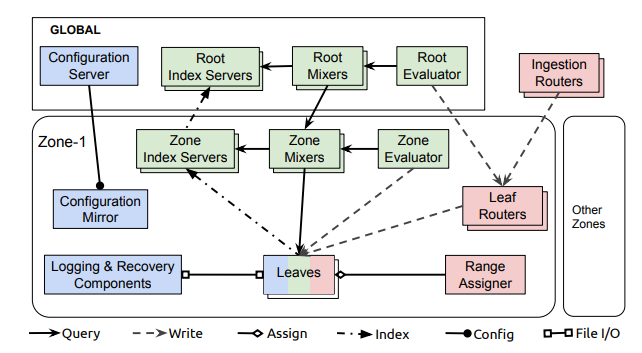
\includegraphics[width=1\textwidth]{pics/monarch.png} % Replace with your image name
    \caption{Overview of Monarch \cite{50652}}
\end{figure}

\subsubsection*{State-Holding Components}

\begin{itemize}
    \item \textbf{Leaves} serve as the primary storage for monitoring data, keeping it in an in-memory time series database.
    \item \textbf{Recovery logs} store monitoring data on disk, mirroring the data held in leaves. Over time, this data is moved into a long-term time series repository.
    \item \textbf{Global configuration server and zonal mirrors} manage configuration data, which is stored in Spanner databases \cite{50652}.
\end{itemize}

\subsubsection*{Data Ingestion Components}

\begin{itemize}
    \item \textbf{Ingestion routers} direct data to leaf routers within the correct Monarch zone, relying on information embedded in time series keys for accurate routing.
    \item \textbf{Leaf routers} receive data bound for a specific zone and forward it to the leaves for storage.
    \item \textbf{Range assigners} handle the distribution of data across leaves, balancing the load within each zone.
\end{itemize}

\subsubsection*{Query Execution Components}

\begin{itemize}
    \item \textbf{Mixers} divide queries into smaller sub-queries routed to and processed by leaves, then combine the results. Queries can be initiated at the root level (handled by root mixers) or at the zone level (handled by zone mixers). Root-level queries require both root and zone mixers.
    \item \textbf{Index servers} provide indexing for each zone and leaf, guiding the distributed execution of queries.
    \item \textbf{Evaluators} periodically execute standing queries (see Section 5.2) by dispatching them to mixers, then write the results back to leaves.
\end{itemize}

\subsection{Data Storage}

Monarch organizes monitoring data into tables that store time series, which are sequences of values recorded over time. Each table includes two main types of columns:

\begin{itemize}
    \item \textbf{Key columns:} These define unique identifiers for each time series, such as the specific machine or service being tracked.
    \item \textbf{Value column:} This stores the historical data points (e.g., memory usage or latency) recorded over time for each time series.
\end{itemize}

Key columns, also referred to as fields, have two sources: targets and metrics.

\subsubsection*{Targets (Monitored Entities)}
\begin{itemize}
    \item A target is the system or component that generates data, like a server, application, or process.
    \item Monarch links each time series to its specific source target, identifying the entity from which the data originates.
    \item Each target follows a schema (template) with specific fields, such as user, job, cluster, or task number for tasks in a computing cluster.
    \item The location field within each target helps Monarch store data near its origin (for instance, data from a specific cluster is stored in the closest zone).
    \item Time series data from the same target are grouped, ensuring related data is stored together and is easier to query.
    \item Target ranges organize targets in alphabetical order to allow efficient data distribution and load balancing, which simplifies group queries.
\end{itemize}

\subsubsection*{Metrics (What We’re Measuring)}
\begin{itemize}
    \item A metric is a specific measurement related to a target, such as the number of requests a server processes or its memory usage.
    \item Each metric has its own schema with particular fields, such as the type of service or command for an RPC request.
    \item Metrics can be various data types, including numbers, strings, or distributions (groups of values that allow for calculations of averages, percentiles, etc.).
\end{itemize}

\subsection{How Data Storage Happens}

The data collection path in Monarch can be broken down into four main steps:

\begin{itemize}
    \item \textbf{Client to Ingestion Router}
    \begin{itemize}
        \item A client application sends time series data to a nearby ingestion router. Monarch's ingestion routers are spread across clusters, allowing data to be gathered close to its origin, thus reducing latency.
        \item Clients frequently utilize Monarch's instrumentation library, which regulates the data write frequency to comply with Monarch's retention policies.
    \end{itemize}
    
    \item \textbf{Ingestion Router to Leaf Router}
    \begin{itemize}
        \item Each ingestion router extracts the location field of the target to determine the appropriate zone for the data, organizing it by geographic or logical regions.
        \item After identifying the target zone, the ingestion router forwards the data to a leaf router within that zone. Zone mappings are dynamically updated.
    \end{itemize}

    \item \textbf{Leaf Router to Leaf Node}
    \begin{itemize}
        \item Within the assigned zone, the leaf router directs data to specific leaf nodes. These leaf nodes manage target ranges, with data sharded lexicographically according to target strings.
        \item Each leaf router keeps an updated range map that indicates which leaf node is responsible for each target range. This map is periodically refreshed by updates from leaf nodes, ensuring uninterrupted data collection even if the range assigner experiences temporary issues.
    \end{itemize}
    
    \item \textbf{Data Storage on Leaf Nodes}
    \begin{itemize}
        \item Upon reaching the assigned leaf node, data is stored in an in-memory time series store and recovery logs. This in-memory store is optimized for efficient handling of timestamp sequences, reducing memory usage.
        \item Data encoding methods, such as \textbf{delta encoding} and \textbf{run-length encoding}, are applied to efficiently manage various time series types, including complex structures like tuples.
    \end{itemize}
\end{itemize}
